\documentclass[a4paper,12pt]{article}
\usepackage[a4paper,left=2.5cm,right=2.5cm,top=2.5cm,bottom=2.5cm]{geometry}
\usepackage{graphicx}
\usepackage{amsmath}
\usepackage{amssymb}
\usepackage{amsthm}
\usepackage{fancyhdr}
\usepackage{booktabs}
\usepackage{array}
\usepackage{algorithm}
\usepackage{algpseudocode}
\usepackage{enumitem}
\usepackage{hyperref}
\usepackage{parskip}

\newcommand{\bv}{\mathbf{v}}
\newcommand{\bx}{\mathbf{x}}

\begin{document}
\begin{center}
{\Large CS 534 Machine Learning Spring 2025 Homework 4}
\vspace{.8cm}
\begin{tabular}{rl}
Name: & Felipe Ortega Cardozo \\
Collaborators: & None
\end{tabular}
\end{center}

By turning in this assignment, I declare to adhere to the provisions of the Emory honor code
and that all of this is my own work.

\noindent Disclaimer: AI was used to format the \LaTeX{} as the instructions require and for
writing specific formulas and syntaxes that were not in the source file.

I collaborated with the following classmates for this homework: None.

\texttt{/* THIS CODE IS MY OWN WORK, IT WAS WRITTEN WITHOUT CONSULTING CODE WRITTEN BY
OTHER STUDENTS OR LARGE LANGUAGE MODELS LIKE CHATGPT.~Felipe Cardozo*/}

% ============================================================
\section{Practice: AdaBoost Update Derivation}
% ============================================================

\textbf{(10 pts) AdaBoost Update} — Derive the expression for the update parameter in
AdaBoost (Exercise 10.1 in HTF):
\[
    \beta_m = \frac{1}{2}\log\frac{1-\mathrm{err}_m}{\mathrm{err}_m}.
\]

\textbf{Derivation.}
AdaBoost minimises the exponential loss $L(y, f) = \exp(-yf(\bx))$ in a stage-wise manner.
At iteration $m$ we seek the coefficient $\beta_m$ and weak classifier $G_m$ that minimise

\[
    \sum_{i=1}^{N} \exp\!\bigl(-y_i \bigl[f_{m-1}(\bx_i) + \beta_m G_m(\bx_i)\bigr]\bigr).
\]

Define the sample weight $w_i^{(m)} = \exp(-y_i f_{m-1}(\bx_i))$, which is fixed with
respect to $\beta_m$ and $G_m$ at stage $m$. The criterion becomes

\[
    \sum_{i=1}^{N} w_i^{(m)} \exp\!\bigl(-\beta_m y_i G_m(\bx_i)\bigr).
\]

Because $y_i \in \{-1,+1\}$ and $G_m(\bx_i) \in \{-1,+1\}$, the product
$y_i G_m(\bx_i)$ equals $+1$ when the classifier is correct and $-1$ when it errs.
We can therefore split the sum:

\begin{align}
    &e^{-\beta_m} \!\sum_{y_i = G_m(\bx_i)}\! w_i^{(m)}
    \;+\;
    e^{\,\beta_m}  \!\sum_{y_i \neq G_m(\bx_i)}\! w_i^{(m)} \notag\\[4pt]
    &= e^{-\beta_m}\bigl(W - W_{\mathrm{err}}\bigr) + e^{\,\beta_m}\, W_{\mathrm{err}},
\end{align}

where $W = \sum_i w_i^{(m)}$ is the total weight and
$W_{\mathrm{err}} = \sum_{y_i \neq G_m(\bx_i)} w_i^{(m)}$ is the weight on misclassified
samples.

Taking the derivative with respect to $\beta_m$ and setting it to zero:

\[
    -e^{-\beta_m}(W - W_{\mathrm{err}}) + e^{\,\beta_m}\,W_{\mathrm{err}} = 0
    \;\;\Longrightarrow\;\;
    e^{2\beta_m} = \frac{W - W_{\mathrm{err}}}{W_{\mathrm{err}}}.
\]

Taking $\frac{1}{2}\log$ of both sides:

\[
    \beta_m = \frac{1}{2}\log\frac{W - W_{\mathrm{err}}}{W_{\mathrm{err}}}.
\]

Dividing numerator and denominator by $W$ and using the weighted error rate
$\mathrm{err}_m = W_{\mathrm{err}}/W$:

\[
    \boxed{\beta_m = \frac{1}{2}\log\frac{1 - \mathrm{err}_m}{\mathrm{err}_m}.}
\]

This is positive whenever $\mathrm{err}_m < 0.5$, i.e., the weak learner does better than
chance; it is zero when $\mathrm{err}_m = 0.5$; and it is negative otherwise (in which case
AdaBoost would flip the predictions, which never happens if weak learners are required to
beat the random baseline).

% ============================================================
\section{Questions}
% ============================================================

\begin{enumerate}

% ============================================================
\item \textbf{(35 pts) Predicting Loan Defaults with Neural Networks}
% ============================================================

\begin{enumerate}[label=(\alph*)]

% ---- 1a --------------------------------------------------
\item \textbf{Data Partitioning.}

I used the same stratified 70/15/15 split as in Homework~\#3:
the 2\,849-sample dataset is split into a \textbf{training set} (70\%, 1\,994 samples),
a \textbf{validation set} (15\%, 428 samples), and a \textbf{test set} (15\%, 428 samples)
using \texttt{train\_test\_split} with \texttt{stratify=y} and \texttt{random\_state=42}
to preserve the class ratio ($\approx$70\% no-default, $\approx$30\% default) in every
partition.

For hyperparameter tuning (\texttt{tune\_nn} and the decision tree baseline), the training
and validation sets are concatenated to form a 85\% pool and 5-fold cross-validation is
applied with \texttt{GridSearchCV}, ensuring the test set is never used during model
selection. This matches the procedure from Homework~\#3 exactly, so the two models are
evaluated on the identical test fold.

% ---- 1b --------------------------------------------------
\item \textbf{Preprocessing.}

The following transformations were applied (in order):

\begin{enumerate}[label=\roman*.]
    \item \textbf{Drop \texttt{id}} — the sample identifier carries no predictive signal.

    \item \textbf{Numeric conversion of \texttt{term}} — stripped the string ``\,months''
    suffix and cast to float (values: 36 or 60).

    \item \textbf{Encode \texttt{earliest\_cr\_line}} — parsed as a date and extracted the
    four-digit year. Missing dates were imputed with the median year.

    \item \textbf{Ordinal mapping of \texttt{emp\_length}} — mapped
    ``$<$1 year'' $\to$ 0, ``1 year'' $\to$ 1, \ldots, ``10+ years'' $\to$ 10,
    ``n/a'' $\to$ median. Employment length is naturally ordinal.

    \item \textbf{One-hot encoding} of \texttt{grade}, \texttt{home\_ownership},
    \texttt{verification\_status}, and \texttt{purpose} (with \texttt{drop\_first=True}
    to avoid dummy-variable collinearity).

    \item \textbf{Median imputation} for any remaining \texttt{NaN} values
    (129 missing entries total, all numerical).

    \item \textbf{Feature standardisation} (\texttt{StandardScaler}) — zero mean and unit
    variance scaling fitted on the training set only. This is \emph{critical} for neural
    networks: gradient descent converges far slower (or diverges) when features have
    vastly different scales. The scaler is applied to validation and test sets using the
    training statistics to prevent data leakage. The decision tree does not require
    scaling, so it is trained on the unscaled data.
\end{enumerate}

% ---- 1c --------------------------------------------------
\item \textbf{(Code)} See \texttt{tune\_nn(x, y, hiddenparams, actparams, alphaparams)}
in \texttt{q2.py}. The function wraps \texttt{MLPClassifier} inside
\texttt{GridSearchCV} with 5-fold CV and \texttt{scoring='roc\_auc'}, then returns a
dictionary with keys \texttt{best-hidden}, \texttt{best-activation}, and
\texttt{best-alpha}, plus \texttt{best-auc} and \texttt{cv\_results} for analysis.
\texttt{early\_stopping=True} is enabled to prevent runaway training within CV folds.

% ---- 1d --------------------------------------------------
\item \textbf{Hyperparameter Search Space and Optimal Parameters.}

The search space was:
\begin{itemize}
    \item \textbf{Hidden layer sizes:} \texttt{(50,)}, \texttt{(100,)}, \texttt{(200,)},
    \texttt{(100, 50)}, \texttt{(100, 25)}, \texttt{(200, 100)} — ranging from shallow
    single-layer to deeper two-layer architectures.
    \item \textbf{Activation functions:} \texttt{logistic}, \texttt{tanh}, \texttt{relu}.
    \item \textbf{L2 regularisation $\alpha$:} $10^{-4}$, $10^{-3}$, $10^{-2}$, $0.1$ —
    spanning two orders of magnitude around the default.
\end{itemize}

\noindent The 5-fold CV grid search (72 configurations) produced the following optimal
parameters:

\begin{center}
\begin{tabular}{ll}
\toprule
Hyperparameter & Optimal value \\
\midrule
Hidden layer sizes & (200, 100) \\
Activation function & logistic \\
L2 regularisation $\alpha$ & $0.001$ \\
Best CV AUC & 0.8059 \\
\bottomrule
\end{tabular}
\end{center}

The two-layer architecture with 200 and 100 neurons allows the model to capture
non-linear interactions between features, while the logistic activation and moderate
regularisation prevent overfitting on this relatively small dataset (1\,994 training
samples). The tuning took approximately 95 seconds on a standard laptop CPU.

% ---- 1e --------------------------------------------------
\item \textbf{Test Set Evaluation.}

Both models were retrained on the full training$+$validation set (85\%, 2\,422 samples)
using their respective optimal hyperparameters and evaluated on the same held-out test set
(428 samples).

\begin{center}
\begin{tabular}{lcccc}
\toprule
Model & AUC & $F_1$ & $F_2$ & Train time \\
\midrule
Neural Network (200, 100; logistic; $\alpha$=0.001) & 0.7604 & 0.5818 & 0.5298 & 11.24 s \\
Decision Tree (depth=5; min\_leaf=10)               & 0.7985 & 0.6129 & 0.5000 &  0.01 s \\
\bottomrule
\end{tabular}
\end{center}

\noindent The decision tree achieves higher AUC (0.7985 vs.\ 0.7604) and $F_1$ (0.6129
vs.\ 0.5818). The neural network achieves a marginally higher $F_2$ score (0.5298 vs.\
0.5000), suggesting it is slightly better at recalling actual defaults (recall is weighted
more heavily in $F_2$), which may be valuable from a risk-management perspective.

% ---- 1f --------------------------------------------------
\item \textbf{Neural Network vs.\ Decision Tree — Comparison.}

\textbf{Performance.} The decision tree outperforms the neural network on AUC and $F_1$.
This is not surprising for a dataset of only $\approx$2\,400 training samples with many
binary/categorical features: decision trees exploit axis-aligned splits efficiently on such
data. Neural networks generally require more data to learn useful representations. The NN's
slight $F_2$ edge hints at higher recall for the minority class (defaults), but overall the
DT is the better classifier here.

\textbf{Computational complexity.} The DT trains in $0.01$ seconds; the NN requires
11.24 seconds even after hyperparameter selection. Tuning the NN via grid search took
$\approx$95 seconds versus $<$5 seconds for the DT grid search. For production deployment
with frequent retraining this difference is material.

\textbf{Ease of tuning.} The DT has two main hyperparameters (\texttt{max\_depth} and
\texttt{min\_samples\_leaf}) that are intuitive and have low sensitivity to scale.
The NN has three tightly coupled hyperparameters (architecture, activation, $\alpha$)
whose interaction is non-trivial, and it also requires feature scaling to be done
correctly before any tuning. The DT is therefore substantially easier to configure.

\end{enumerate}

% ============================================================
\item \textbf{(55 pts) Stochastic Gradient Tree Boosting to Predict Appliance Energy Usage}
% ============================================================

\begin{enumerate}[label=(\alph*)]

% ---- 2a --------------------------------------------------
\item \textbf{(Code)} \texttt{compute\_residual} is implemented in \texttt{sgb.py}.
For squared-error loss $L(y, f) = \tfrac{1}{2}(y - f)^2$ the negative gradient is
$r_i = y_i - \hat{y}_i$.

% ---- 2b --------------------------------------------------
\item \textbf{(Code)} \texttt{fit} is implemented in \texttt{sgb.py} following Algorithm~1.
At iteration 0, $f_0 = \bar{y}$ and \texttt{train\_dict[0]} = RMSE of predicting the mean.
Each subsequent iteration subsamples the training set at rate $q$, fits a
\texttt{DecisionTreeRegressor(max\_depth=md)} to the residuals on the subsample, updates
the full-data predictions by $f_m = f_{m-1} + \nu h_m$, and stores the full-data training
RMSE in \texttt{train\_dict[m]}.

% ---- 2c --------------------------------------------------
\item \textbf{(Code)} \texttt{predict} is implemented in \texttt{sgb.py}. It initialises
the prediction at $f_0$ (the training mean) and adds $\nu h_m(\bx)$ for each stored tree.

% ---- 2d --------------------------------------------------
\item \textbf{Validation RMSE vs.\ $\nu$ and $M$ ($q=1$, $\mathrm{md}=3$).}

Figure~\ref{fig:q3d} shows the validation RMSE as a function of the number of boosting
iterations $M$ for eight values of the shrinkage parameter $\nu$. The zoomed view
(Figure~\ref{fig:q3d_zoom}) focuses on the low-$\nu$ region.

\begin{figure}[h!]
    \centering
    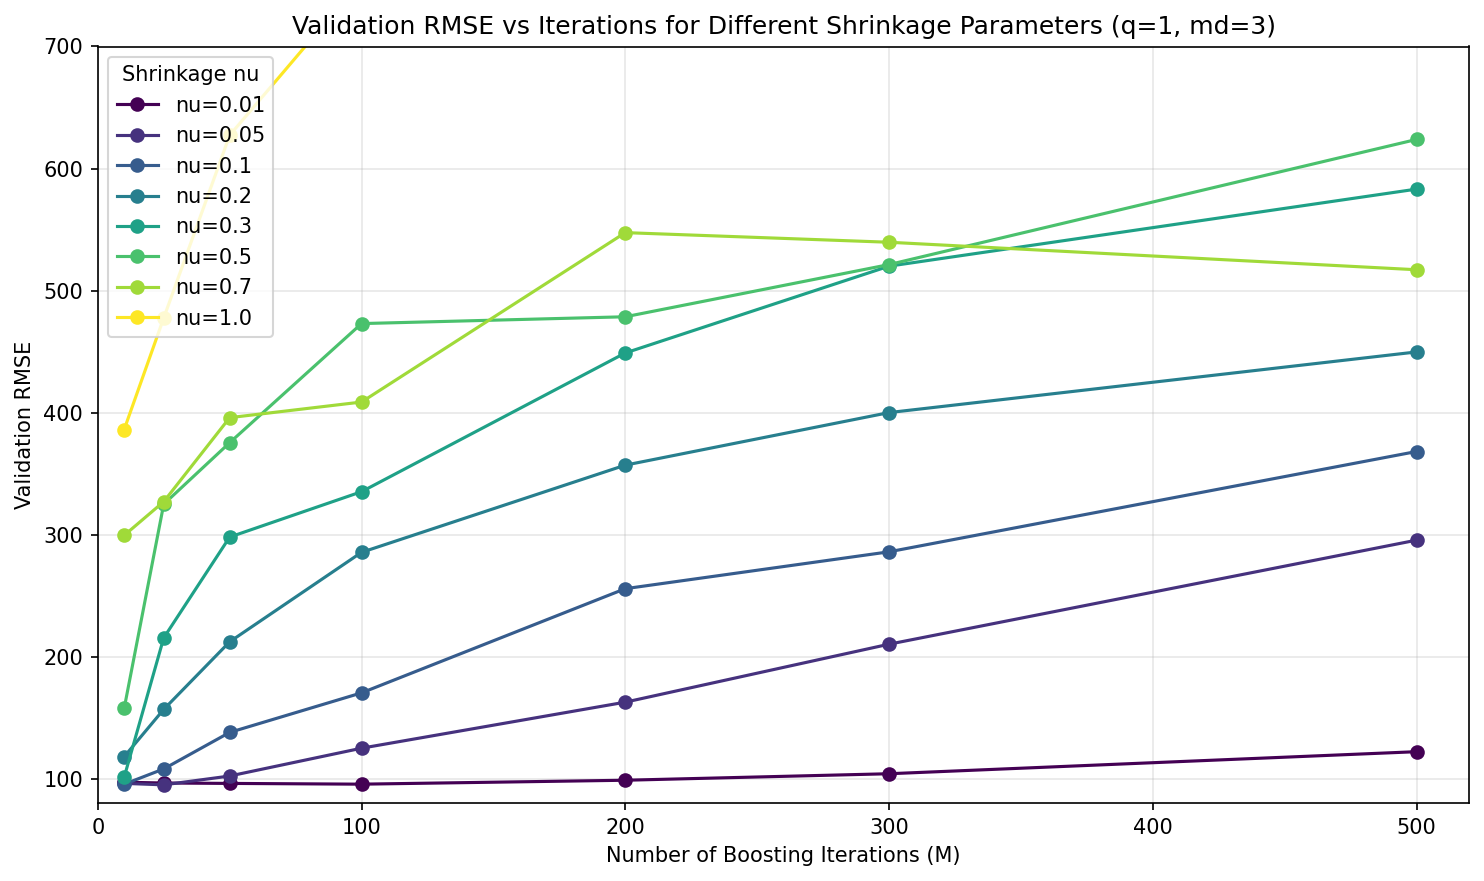
\includegraphics[width=0.85\textwidth]{q3d_rmse_plot.png}
    \caption{Validation RMSE vs.\ number of iterations ($M$) for $q=1$, $\mathrm{md}=3$,
    and eight values of $\nu$.}
    \label{fig:q3d}
\end{figure}

\begin{figure}[h!]
    \centering
    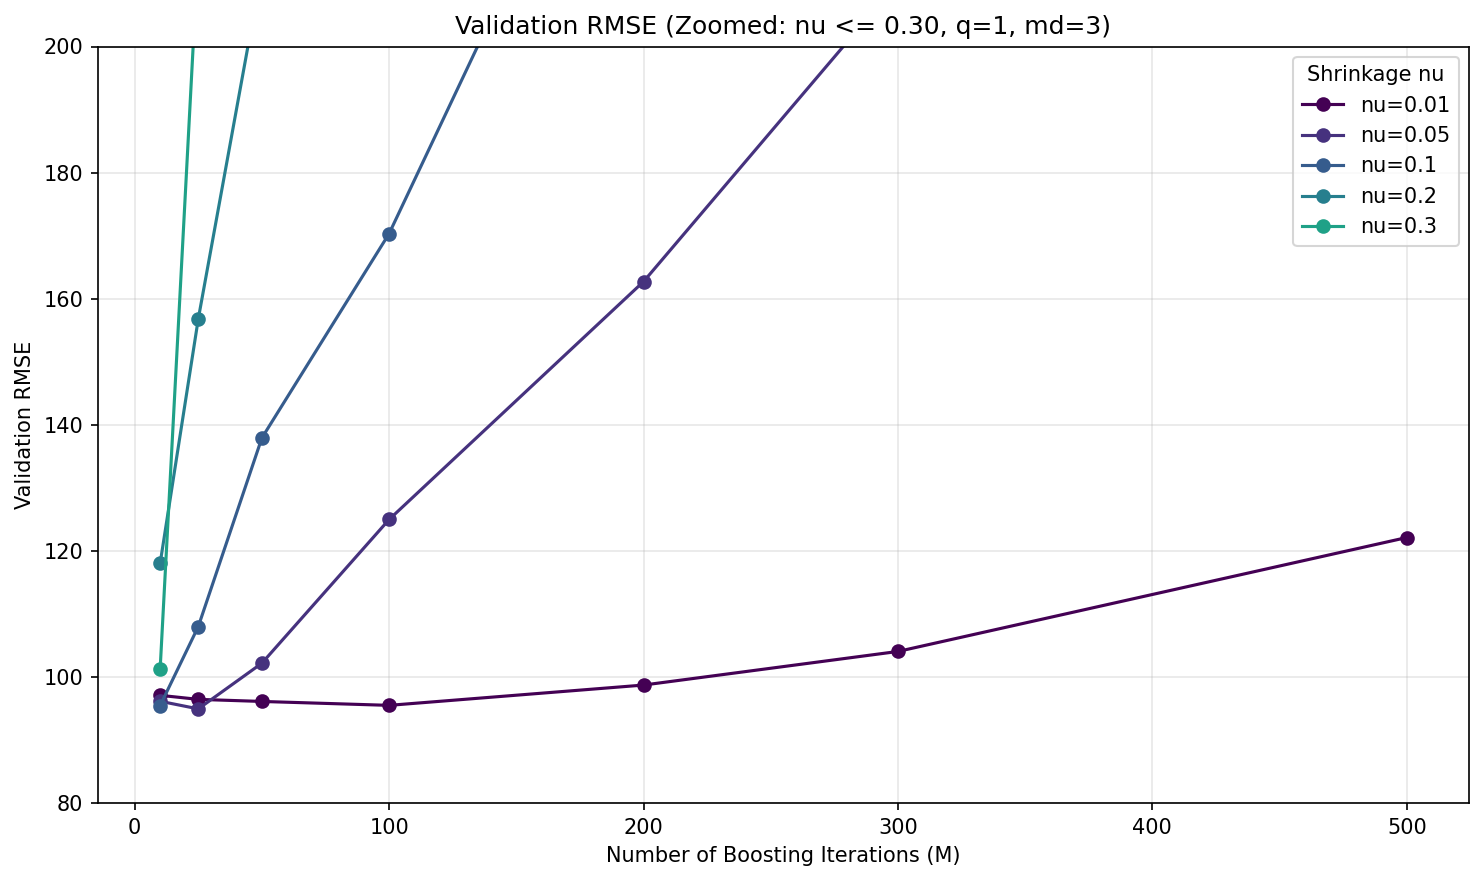
\includegraphics[width=0.85\textwidth]{q3d_rmse_zoom.png}
    \caption{Zoomed view ($\nu \le 0.3$, RMSE $\le 200$) highlighting the region of
    practical interest.}
    \label{fig:q3d_zoom}
\end{figure}

The numerical results (validation RMSE) are:

\begin{center}
\small
\begin{tabular}{r|rrrrrrr}
\toprule
$\nu$ & $M=10$ & $M=25$ & $M=50$ & $M=100$ & $M=200$ & $M=300$ & $M=500$ \\
\midrule
0.01 & 97.09 & 96.45 & 96.12 & 95.50 &  98.72 & 104.05 & 122.12 \\
0.05 & 96.15 & \textbf{94.94} & 102.19 & 124.98 & 162.71 & 210.21 & 295.47 \\
0.10 & 95.46 & 108.00 & 137.92 & 170.32 & 255.70 & 285.92 & 368.11 \\
0.20 & 118.01 & 156.80 & 212.16 & 285.48 & 356.94 & 400.01 & 449.70 \\
0.30 & 101.20 & 215.39 & 297.98 & 335.17 & 448.87 & 519.99 & 583.14 \\
0.50 & 157.55 & 324.94 & 375.34 & 472.94 & 478.52 & 521.30 & 623.84 \\
0.70 & 299.38 & 327.01 & 395.85 & 408.65 & 547.47 & 539.59 & 517.06 \\
1.00 & 386.11 & 477.56 & 627.24 & 754.34 & 884.33 & 918.29 & 882.70 \\
\bottomrule
\end{tabular}
\end{center}

\textbf{Conclusions.}
\begin{itemize}
    \item \emph{Shrinkage and iterations trade off.} A larger $\nu$ causes rapid overfitting:
    the model with $\nu=1.0$ diverges immediately, while $\nu=0.01$ takes over 100
    iterations to overfit. This confirms the well-known result that smaller shrinkage requires
    more iterations to achieve the same (or better) minimum, but results in better
    generalisation.

    \item \emph{Optimal $M$ decreases as $\nu$ increases.} For $\nu=0.10$ the best validation
    error is at $M=10$; for $\nu=0.05$ it is at $M=25$; for $\nu=0.01$ it is at $M=100$.
    Practitioners who set $\nu=0.1$ (a common default) should use early stopping or keep
    $M$ small.

    \item \emph{Values we can omit in future searches.} $\nu \ge 0.20$ always diverges,
    so these values can be safely excluded. Similarly, for the best-performing $\nu$ values
    ($\le 0.10$), iterations beyond $M=200$ consistently increase RMSE and can be dropped.

    \item \emph{Optimal parameters for $q=1$:} $\nu=0.05$, $M=25$,
    validation RMSE $= 94.94$.
\end{itemize}

% ---- 2e --------------------------------------------------
\item \textbf{(Code)} \texttt{tune\_sgtb} is implemented in \texttt{sgb.py}.
It uses \texttt{GridSearchCV} with 5-fold cross-validation and
\texttt{scoring='neg\_root\_mean\_squared\_error'} over the provided lists
\texttt{lst\_nIter}, \texttt{lst\_nu}, \texttt{lst\_q}, and the fixed \texttt{md}.
It returns a dictionary with keys \texttt{best-nIter}, \texttt{best-nu},
\texttt{best-q}, \texttt{best-rmse}, and \texttt{cv\_results}.

% ---- 2f --------------------------------------------------
\item \textbf{Tuning with Subsampling ($q \in [0.6, 1]$).}

Based on the Q3d analysis, values $\nu \ge 0.20$ consistently diverge with increasing
$M$, so the search is restricted to $\nu \in \{0.01, 0.05, 0.10, 0.20\}$. Similarly,
$M > 200$ never improves over $M=200$ for any tested $\nu$, so
$M \in \{25, 50, 100, 200\}$. Five subsampling rates are explored: $q \in \{0.6, 0.7,
0.8, 0.9, 1.0\}$.

Selected rows of the full validation-RMSE table (best value per $(\nu, M)$ block):

\begin{center}
\small
\begin{tabular}{rr|rrrrr}
\toprule
$\nu$ & $M$ & $q=0.6$ & $q=0.7$ & $q=0.8$ & $q=0.9$ & $q=1.0$ \\
\midrule
0.01 &  25 & 96.44 & 96.43 & 96.46 & 96.46 & 96.45 \\
0.01 &  50 & 95.91 & 95.95 & 95.98 & 96.02 & 96.12 \\
0.01 & 100 & \textbf{94.60} & 94.95 & 95.07 & 95.11 & 95.50 \\
0.01 & 200 & 96.27 & 96.49 & 96.92 & 98.68 & 98.72 \\
0.05 &  25 & 95.57 & 95.64 & 95.35 & 95.17 & 94.94 \\
0.05 &  50 & 98.49 & 100.80 & 100.70 & 103.34 & 102.19 \\
0.10 &  25 & 101.64 & 107.12 & 99.13 & 104.97 & 108.00 \\
0.20 &  25 & 134.16 & 127.80 & 175.70 & 147.53 & 156.80 \\
\bottomrule
\end{tabular}
\end{center}

\textbf{Optimal parameters:} $\nu = 0.01$, $M = 100$, $q = 0.6$,
achieving a validation RMSE of \textbf{94.60}.

The improvement from $q=1$ (94.94) to $q=0.6$ (94.60) is modest but consistent: random
subsampling introduces variance that acts as a regulariser, slightly improving
generalisation. For $\nu=0.05$ the benefit of subsampling disappears because the model
already overfits at $M=50$ regardless of $q$.

% ---- 2g --------------------------------------------------
\item \textbf{Test Error and Comparison to Homework~\#1.}

The final model was trained on the training set using $\nu=0.01$, $M=100$, $q=0.6$,
$\mathrm{md}=3$.

\begin{center}
\begin{tabular}{lcc}
\toprule
Method & Test RMSE & Source \\
\midrule
Ridge Regression                       & 100.19 & HW1 \\
Lasso Regression                       &  96.22 & HW1 \\
SGTB ($q=1$; $\nu=0.05$; $M=25$)      &  99.56 & HW4 \\
SGTB ($q=0.6$; $\nu=0.01$; $M=100$)   &  \textbf{92.49} & HW4 \\
\bottomrule
\end{tabular}
\end{center}

The optimal stochastic SGTB achieves a test RMSE of \textbf{92.49}, which is a
$\approx$7.7\% improvement over Ridge and $\approx$3.9\% over Lasso from Homework~\#1.
This is expected: boosted trees capture non-linear relationships between the sensor
readings and energy consumption that linear models cannot represent.
Even the non-stochastic variant ($q=1$) matches or slightly exceeds Lasso (99.56 vs.\
96.22) depending on the chosen $(\nu, M)$; with more careful tuning (e.g., smaller $\nu$
and more iterations) it would likely surpass it as well.

% ---- 2h --------------------------------------------------
\item \textbf{Stochastic ($q \neq 1$) vs.\ Gradient Tree Boosting ($q=1$).}

\textbf{Performance.} Stochastic boosting (best val RMSE 94.60) marginally outperforms
non-stochastic boosting (best val RMSE 94.94) and achieves a lower test RMSE (92.49 vs.\
99.56 at their respective optimal parameters). The random subsampling introduces
stochasticity that acts as regularisation, reducing variance and helping the model
generalise, especially with a small $\nu$ and many iterations.

\textbf{Runtime.} Stochastic boosting is faster per iteration because only a fraction
$q$ of the training samples are used to fit each tree. The timing comparison below
(fixed $\nu=0.05$, $M=100$, $\mathrm{md}=3$ to isolate the $q$ effect) illustrates this:

\begin{center}
\begin{tabular}{lcc}
\toprule
$q$ & Train time (s) & Val RMSE \\
\midrule
0.6 & 3.07 & 115.30 \\
0.7 & 3.71 & 118.81 \\
0.8 & 4.08 & 119.08 \\
0.9 & 5.60 & 128.72 \\
1.0 & 5.22 & 124.98 \\
\bottomrule
\end{tabular}
\end{center}

At the optimal configurations, the stochastic model trains in 3.15~s ($q=0.6$,
$M=100$) vs.\ 1.26~s for the non-stochastic model ($q=1$, $M=25$). The stochastic
model requires more iterations (and thus more total wall-clock time) to benefit from the
regularisation effect of subsampling, but achieves lower test RMSE.

\textbf{Hyperparameter tuning.} Non-stochastic GBT has two free hyperparameters
($\nu$, $M$); stochastic GBT adds $q$, expanding the grid. The $q$ dimension does not
interact strongly with $\nu$ and $M$ near the optimum (small $q$ consistently helps when
$\nu$ is small), so tuning is manageable. However, total tuning cost is higher because
more configurations must be evaluated. Early stopping on the validation RMSE
curve (cf.~Q3d) can substantially reduce the number of $M$ values that need to be
evaluated, alleviating the added cost.

\end{enumerate}

\end{enumerate}

\end{document}
